\chapter{Introduction and Background}

\section{About this Template}
This template is an adaptation \texttt{gatechthesis\_latex} template (17 January 2017 update) and \texttt{ut-diss-2}. 
I've made some (mostly) aesthetic changes, but I believe it should conform to the requirements liseted in the Georgia Tech ``Graduate Thesis/Dissertation Guidelines \& Procedures'' (April 2015 Update).
It is by no means an official template, though. 
So as stated in the license file, you can use, change, distribute, sell it however you'd like, provided
\begin{enumerate}
  \item You include the copyright notice in the license file; and
  \item You hold none of the authors liable for any results of such use.
\end{enumerate}

\section{Basic Elements}
This section talks about common components (figures, tables, and equations), and how they're included in \LaTeX{} documents.
Much better and more complete resources are available elsewhere, but hopefully this enough to get started.

\subsection{Figures}
Figures are included with the \texttt{figure} environment.
They are floats, which means that they will appear wherever \LaTeX{} thinks is best based on the surrounding text.
You can tinker with this positioning, but the details are out of scope.
A quick example will give most of the salient details. 
The following code will give the results in \cref{fig:IntensityVsWavelength}.
\begin{minipage}{0.75\textwidth}
\footnotesize
  \vspace{2mm}
  \begin{verbatim}
\begin{figure}
  \centering
  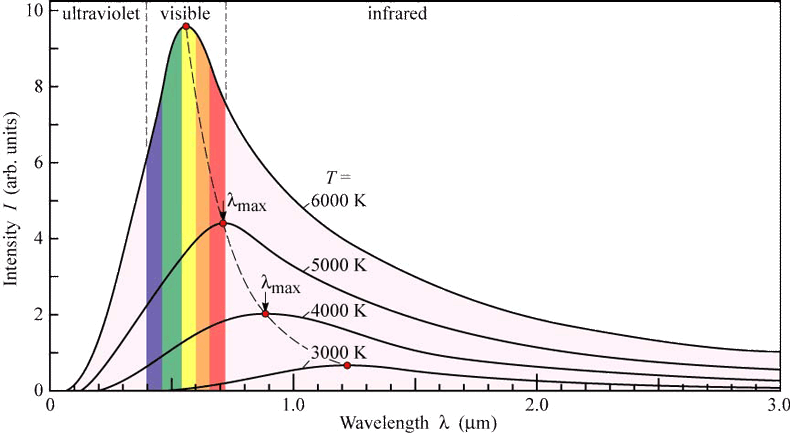
\includegraphics[width=0.75\linewidth]{figures/exampleFigure.png}
  \caption[Short Caption]{This is a long caption. It's too long  
         for the table of contents, so we specify a short caption 
         in the brackets.}
  \label{fig:IntensityVsWavelength}
\end{figure}
  \end{verbatim}
  \vspace{2mm}
\end{minipage}

Note the use of a short caption in brackets in the \texttt{\textbackslash caption} command.
This lets us have a long explanatory caption, without keeping our List of Tables compact (compare the caption of \cref{fig:IntensityVsWavelength}) with how it's listed on \cpageref{sec:ListOfTables}.

\begin{figure}
  \centering
  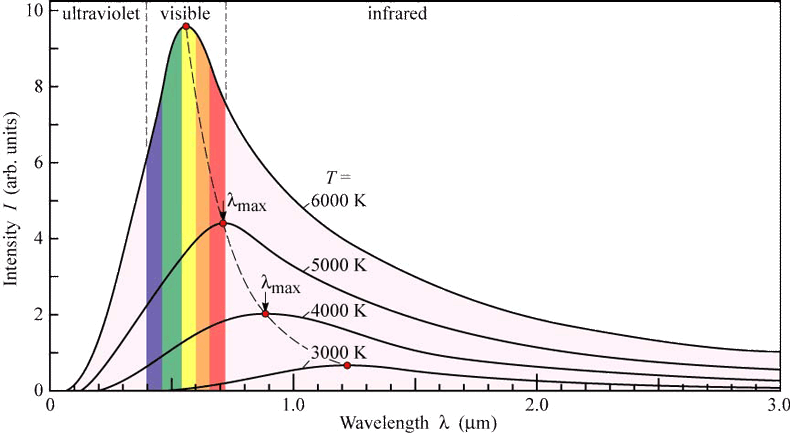
\includegraphics[width=0.75\linewidth]{figures/exampleFigure.png}
  \caption[Short Caption]{This is a long caption. It's too long  
         for the table of contents, so we specify a short caption 
         in the brackets.}
  \label{fig:IntensityVsWavelength}
\end{figure}

\subsection{Tables}


\subsection{Equations}
I recommend using the \texttt{align} environment exclusively for equations. 
It's virtually identical to \texttt{equation}, but allows you to have multiple lines and specify where you want them to---well---\emph{align} with each other.
Compare the following\\
\begin{minipage}[t]{0.48\textwidth}
\small
\begin{verbatim}
\begin{equation}
  a^{2} + b^{2} = c^{2}
\end{equation}
\end{verbatim}
\begin{equation}
  a^{2} + b^{2} = c^{2}
\end{equation}
\end{minipage}
~
\begin{minipage}[t]{0.48\textwidth}
\small
\begin{verbatim}
\begin{align}
  a^{2} + b^{2} = c^{2}
\end{align}
\end{verbatim}
\begin{align}
  a^{2} + b^{2} = c^{2}
\end{align}
\end{minipage}


\section{Cross-Referencing}
One of the chief advantages of \LaTeX{} is how easy it makes cross-references.
Note that we often want to refer to a figure or equation.
Sure, we could number them by hand, but it we insert or delete 


Items are referenced using \texttt{cleveref} and \texttt{hyperref} packages. For example, here's an equation
\begin{align}
   i\hbar\frac{\partial}{\partial t}\Psi &= \left[ \frac{-\hbar^{2}}{2m}\nabla^{2} + V\right]\Psi\,.
  \label{eqn:SchrodingerEquation}
\end{align}
\Cref{eqn:SchrodingerEquation} should be referenced as so.

Lorem ipsum dolor sit amet, consectetur adipiscing elit, sed do eiusmod tempor incididunt ut labore et dolore magna aliqua. Ut enim ad minim veniam, quis nostrud exercitation ullamco laboris nisi ut aliquip ex ea commodo consequat \cite{ref1}. Duis aute irure dolor in reprehenderit in voluptate velit esse cillum dolore eu fugiat nulla pariatur \cite{ref2}. Excepteur sint occaecat cupidatat non proident, sunt in culpa qui officia deserunt mollit anim id est laborum.

Lorem ipsum dolor sit amet, consectetur adipiscing elit, sed do eiusmod tempor incididunt ut labore et dolore magna aliqua. Ut enim ad minim veniam, quis nostrud exercitation ullamco laboris nisi ut aliquip ex ea commodo consequat \cite{ref1}. Duis aute irure dolor in reprehenderit in voluptate velit esse cillum dolore eu fugiat nulla pariatur \cite{ref2}. Excepteur sint occaecat cupidatat non proident, sunt in culpa qui officia deserunt mollit anim id est laborum.

Lorem ipsum dolor sit amet, consectetur adipiscing elit, sed do eiusmod tempor incididunt ut labore et dolore magna aliqua. Ut enim ad minim veniam, quis nostrud exercitation ullamco laboris nisi ut aliquip ex ea commodo consequat \cite{ref1}. Duis aute irure dolor in reprehenderit in voluptate velit esse cillum dolore eu fugiat nulla pariatur \cite{ref2}. Excepteur sint occaecat cupidatat non proident, sunt in culpa qui officia deserunt mollit anim id est laborum.

Lorem ipsum dolor sit amet, consectetur adipiscing elit, sed do eiusmod tempor incididunt ut labore et dolore magna aliqua. Ut enim ad minim veniam, quis nostrud exercitation ullamco laboris nisi ut aliquip ex ea commodo consequat \cite{ref1}. Duis aute irure dolor in reprehenderit in voluptate velit esse cillum dolore eu fugiat nulla pariatur \cite{ref2}. Excepteur sint occaecat cupidatat non proident, sunt in culpa qui officia deserunt mollit anim id est laborum.

Lorem ipsum dolor sit amet, consectetur adipiscing elit, sed do eiusmod tempor incididunt ut labore et dolore magna aliqua. Ut enim ad minim veniam, quis nostrud exercitation ullamco laboris nisi ut aliquip ex ea commodo consequat \cite{ref1}. Duis aute irure dolor in reprehenderit in voluptate velit esse cillum dolore eu fugiat nulla pariatur \cite{ref2}. Excepteur sint occaecat cupidatat non proident, sunt in culpa qui officia deserunt mollit anim id est laborum.

% This is a table

\begin{table}
\caption{This is an example Table.}
\begin{center}
\begin{tabular}{ccc}
$x$ & $f(x)$ & $g(x)$ \\
\hline
1 & 6 & 4  \\
2 & 6 & 3  \\
3 & 6 & 2  \\
4 & 6 & 2  \\
\label{tab:ValuesOfFunctions}
\end{tabular}
\end{center}
\end{table}
